% Für Bindekorrektur als optionales Argument "BCORfaktormitmaßeinheit", dann
% sieht auch Option "twoside" vernünftig aus
% Näheres zu "scrartcl" bzw. "scrreprt" und "scrbook" siehe KOMA-Skript Doku
\documentclass[12pt,a4paper,headinclude,bibtotoc]{scrartcl}


%---- Allgemeine Layout Einstellungen ------------------------------------------

% Für Kopf und Fußzeilen, siehe auch KOMA-Skript Doku
\usepackage[komastyle]{scrpage2}
\pagestyle{scrheadings}
\automark[section]{chapter}
\setheadsepline{0.5pt}[\color{black}]

%keine Einrückung
\parindent0pt

%Einstellungen für Figuren- und Tabellenbeschriftungen
\setkomafont{captionlabel}{\sffamily\bfseries}
\setcapindent{0em}

\usepackage{caption}

%---- Weitere Pakete -----------------------------------------------------------
% Die Pakete sind alle in der TeX Live Distribution enthalten. Wichtige Adressen
% www.ctan.org, www.dante.de

% Sprachunterstützung
\usepackage[ngerman]{babel}

% Benutzung von Umlauten direkt im Text
% entweder "latin1" oder "utf8"
\usepackage[utf8]{inputenc}

% Pakete mit Mathesymbolen und zur Beseitigung von Schwächen der Mathe-Umgebung
\usepackage{latexsym,exscale,amssymb,amsmath}

% Weitere Symbole
\usepackage[nointegrals]{wasysym}
\usepackage{eurosym}

% Anderes Literaturverzeichnisformat
%\usepackage[square,sort&compress]{natbib}

% Für Farbe
\usepackage{color}

% Zur Graphikausgabe
%Beipiel: \includegraphics[width=\textwidth]{grafik.png}
\usepackage{graphicx}

% Text umfließt Graphiken und Tabellen
% Beispiel:
% \begin{wrapfigure}[Zeilenanzahl]{"l" oder "r"}{breite}
%   \centering
%   \includegraphics[width=...]{grafik}
%   \caption{Beschriftung} 
%   \label{fig:grafik}
% \end{wrapfigure}
\usepackage{wrapfig}

% Mehrere Abbildungen nebeneinander
% Beispiel:
% \begin{figure}[htb]
%   \centering
%   \subfigure[Beschriftung 1\label{fig:label1}]
%   {\includegraphics[width=0.49\textwidth]{grafik1}}
%   \hfill
%   \subfigure[Beschriftung 2\label{fig:label2}]
%   {\includegraphics[width=0.49\textwidth]{grafik2}}
%   \caption{Beschriftung allgemein}
%   \label{fig:label-gesamt}
% \end{figure}
\usepackage{subfigure}
\usepackage{adjustbox}

% Caption neben Abbildung
% Beispiel:
% \sidecaptionvpos{figure}{"c" oder "t" oder "b"}
% \begin{SCfigure}[rel. Breite (normalerweise = 1)][hbt]
%   \centering
%   \includegraphics[width=0.5\textwidth]{grafik.png}
%   \caption{Beschreibung}
%   \label{fig:}
% \end{SCfigure}
\usepackage{sidecap}

% Befehl für "Entspricht"-Zeichen
\newcommand{\corresponds}{\ensuremath{\mathrel{\widehat{=}}}}

%Für chemische Formeln (von www.dante.de)
%% Anpassung an LaTeX(2e) von Bernd Raichle
\makeatletter
\DeclareRobustCommand{\chemical}[1]{%
  {\(\m@th
   \edef\resetfontdimens{\noexpand\)%
       \fontdimen16\textfont2=\the\fontdimen16\textfont2
       \fontdimen17\textfont2=\the\fontdimen17\textfont2\relax}%
   \fontdimen16\textfont2=2.7pt \fontdimen17\textfont2=2.7pt
   \mathrm{#1}%
   \resetfontdimens}}
\makeatother

%Si Einheiten
\usepackage{siunitx}

%c++ Code einbinden
\usepackage{listings}
\lstset{numbers=left, numberstyle=\tiny, numbersep=5pt}

%Differential
\newcommand{\dif}{\ensuremath{\mathrm{d}}}

%Boxen,etc.
\usepackage{fancybox}
\usepackage{empheq}

%Fußnoten auf gleiche Seite
\interfootnotelinepenalty=1000

%Dateien aus Unterverzeichnissen
\usepackage{import}

%Bibliography \bibliography{literatur} und \cite{gerthsen}
%\usepackage{cite}
\usepackage{babelbib}
\selectbiblanguage{ngerman}

\begin{document}

\title{Wetter}
\author{Felix Kurtz}
\maketitle

\section{Lokales Wetter}
Am Versuchstag, dem 07.12.15, herrschte in Göttingen mildes Wetter mit Temperaturen rund um die $10\si{\celsius}$.
Die Wolken waren größtenteils \textit{Stratus}-Wolken, die den Himmel großflächig bedeckten.
In einigen Wolkenlöchern konnte man \textit{Altocumulus}-Wolken entdecken.
Außerdem war es fast windstill. 
Dies lässt keine schnelle Wetteränderung erkennen, da die Wolken sich somit kaum bewegen.
Die Wolkenschicht reißt höchstens ein bisschen auf oder es beginnt leicht zu regnen.

\section{Wettervorhersage}
Am 07.12. befand sich ein großes Hochdruckgebiet über Zentraleuropa, welches mit bis zu $1040\,$hPa ziemlich stark und somit stabil war (vgl, Abb.\ref{fig:wetter7}).
Dies sorgte für das ungewöhnlich milde Wetter, denn so kam feuchte, warme Mittelmeerluft nach Deutschland.
Die beobachtete Windstille kann man auch aus der Druckkarte ablesen, da die Isobaren über Deutschland weit auseinander liegen.
Die Tiefdruckgebiete südlich von Island und über Russland werden sich vermutlich zu einem Gebiet vereinigen (vgl. Abb.\ref{fig:wetter12}).
Dabei wird allerdings keine Kaltfront über Deutschland ziehen, da das Hoch sehr ausgeprägt ist.
Anhand der anderen Karten in Abbildung \ref{fig:wettervorhersage} kann man erkennen, dass sich das Hoch über Mitteleuropa hält und das Wetter somit mild bleibt, da die Luft weiterhin aus dem Südwesten kommt.
Wir prophezeiten, dass es kurz vor Weihnachten zu einem kleinen Wintereinbruch kommen könnte, da dann laut der Vorhersage die Isobaren in Nord-Süd-Richtung sind und so skandinavische Luft nach Deutschland kommen kann.
Dies erfüllte sich nicht,jedoch war es auch eine sehr langfristige Prognose, sodass den Druckkarten dieses Zeitraums nicht so viel Bedeutung zugemessen werden sollte.


 \begin{figure}[!htb]
   \centering
   \subfigure[7.12.\label{fig:wetter7}]
   {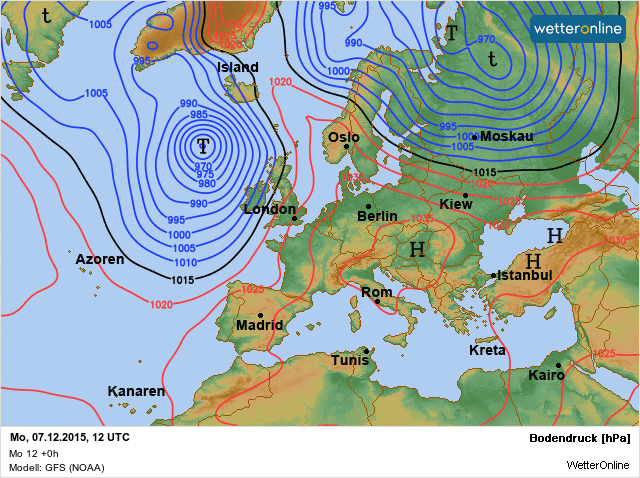
\includegraphics[width=0.49\textwidth]{wetter0712.png}}
   \hfill
   \subfigure[12.12.\label{fig:wetter12}]
   {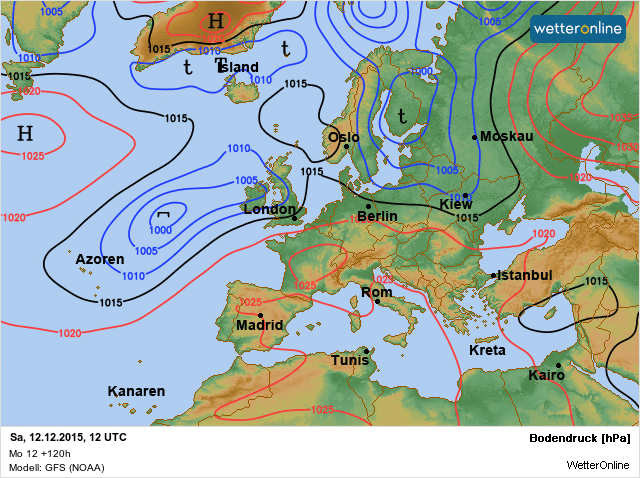
\includegraphics[width=0.49\textwidth]{wetter1212.png}}
   \hfill	
	\subfigure[16.12.\label{fig:wetter16}]
   {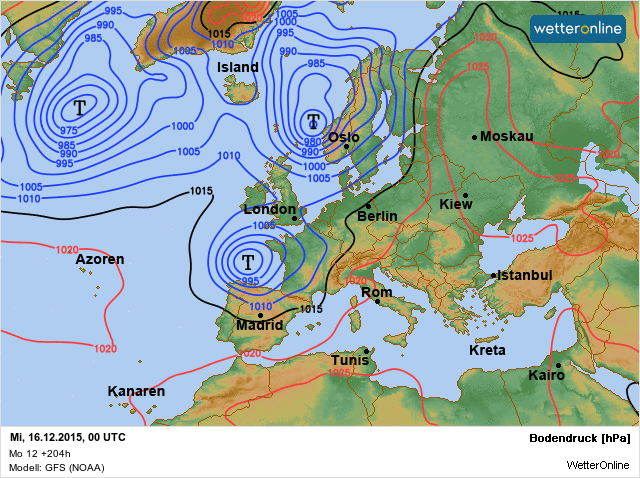
\includegraphics[width=0.49\textwidth]{wetter1612.png}}
   \hfill
   \subfigure[19.12.\label{fig:wetter19}]
   {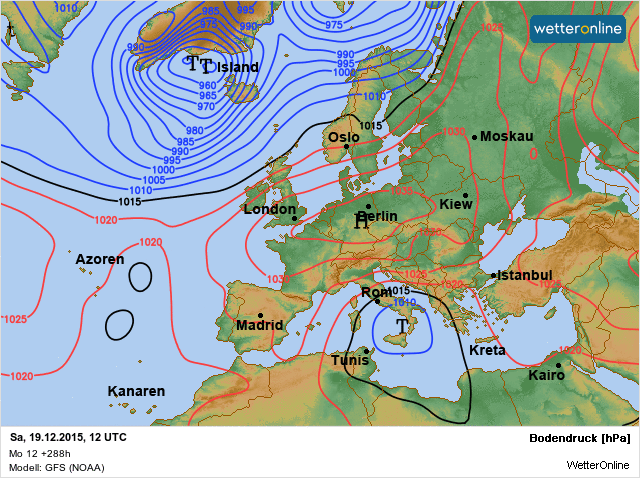
\includegraphics[width=0.49\textwidth]{wetter1912.png}}   
   \caption{Bodendruckkarten/-vorhersagen vom 07.12.15 von \texttt{wetteronline.de}}
   \label{fig:wettervorhersage}
 \end{figure}

\section{Relation Druck und Höhe}
Mit einem Absolutdruck-Messgerät soll das Barometrische Höhengesetz verifiziert werden.
Dazu misst man den Druck sowie die Höhe an verschiedenen Punkten im DLR-SchoolLab.
In Abb.\ref{fig:druckHoehe} sind diese Werte eingetragen.
Der Druck ist dort allerdings nur relativ angegeben: $\Delta p = p-p_0$ mit $p_0=p(0\,\si{m})=1014.035\,$hPa.
Die Messungenauigkeiten sind $\sigma_h=5\,$cm und $\sigma_p=0.05\,$hPa.
Aus der linearen Regression der Messwerte erhält man eine Geradensteigung von $m=(-0.123 \pm 0.013)\,\si{\hecto\pascal\per\meter}$.
Dies bedeutet, dass der Druck etwa um $1\,$hPa auf $8\,$Metern abnimmt.
Das ist der in der Vorlesung angegebene Wert.
Damit lassen sich allerdings nur Druckunterschiede für geringe Höhen(-unterschiede) beschreiben, da der Druck exponentiell abnimmt und dies nur die Linearisierung in Meereshöhe ist.
\begin{figure}[!htb]
	\centering
	\begin{minipage}{0.7\textwidth}
		\resizebox{\textwidth}{!}{   		
   		% GNUPLOT: LaTeX picture with Postscript
\begingroup
  \makeatletter
  \providecommand\color[2][]{%
    \GenericError{(gnuplot) \space\space\space\@spaces}{%
      Package color not loaded in conjunction with
      terminal option `colourtext'%
    }{See the gnuplot documentation for explanation.%
    }{Either use 'blacktext' in gnuplot or load the package
      color.sty in LaTeX.}%
    \renewcommand\color[2][]{}%
  }%
  \providecommand\includegraphics[2][]{%
    \GenericError{(gnuplot) \space\space\space\@spaces}{%
      Package graphicx or graphics not loaded%
    }{See the gnuplot documentation for explanation.%
    }{The gnuplot epslatex terminal needs graphicx.sty or graphics.sty.}%
    \renewcommand\includegraphics[2][]{}%
  }%
  \providecommand\rotatebox[2]{#2}%
  \@ifundefined{ifGPcolor}{%
    \newif\ifGPcolor
    \GPcolorfalse
  }{}%
  \@ifundefined{ifGPblacktext}{%
    \newif\ifGPblacktext
    \GPblacktexttrue
  }{}%
  % define a \g@addto@macro without @ in the name:
  \let\gplgaddtomacro\g@addto@macro
  % define empty templates for all commands taking text:
  \gdef\gplbacktext{}%
  \gdef\gplfronttext{}%
  \makeatother
  \ifGPblacktext
    % no textcolor at all
    \def\colorrgb#1{}%
    \def\colorgray#1{}%
  \else
    % gray or color?
    \ifGPcolor
      \def\colorrgb#1{\color[rgb]{#1}}%
      \def\colorgray#1{\color[gray]{#1}}%
      \expandafter\def\csname LTw\endcsname{\color{white}}%
      \expandafter\def\csname LTb\endcsname{\color{black}}%
      \expandafter\def\csname LTa\endcsname{\color{black}}%
      \expandafter\def\csname LT0\endcsname{\color[rgb]{1,0,0}}%
      \expandafter\def\csname LT1\endcsname{\color[rgb]{0,1,0}}%
      \expandafter\def\csname LT2\endcsname{\color[rgb]{0,0,1}}%
      \expandafter\def\csname LT3\endcsname{\color[rgb]{1,0,1}}%
      \expandafter\def\csname LT4\endcsname{\color[rgb]{0,1,1}}%
      \expandafter\def\csname LT5\endcsname{\color[rgb]{1,1,0}}%
      \expandafter\def\csname LT6\endcsname{\color[rgb]{0,0,0}}%
      \expandafter\def\csname LT7\endcsname{\color[rgb]{1,0.3,0}}%
      \expandafter\def\csname LT8\endcsname{\color[rgb]{0.5,0.5,0.5}}%
    \else
      % gray
      \def\colorrgb#1{\color{black}}%
      \def\colorgray#1{\color[gray]{#1}}%
      \expandafter\def\csname LTw\endcsname{\color{white}}%
      \expandafter\def\csname LTb\endcsname{\color{black}}%
      \expandafter\def\csname LTa\endcsname{\color{black}}%
      \expandafter\def\csname LT0\endcsname{\color{black}}%
      \expandafter\def\csname LT1\endcsname{\color{black}}%
      \expandafter\def\csname LT2\endcsname{\color{black}}%
      \expandafter\def\csname LT3\endcsname{\color{black}}%
      \expandafter\def\csname LT4\endcsname{\color{black}}%
      \expandafter\def\csname LT5\endcsname{\color{black}}%
      \expandafter\def\csname LT6\endcsname{\color{black}}%
      \expandafter\def\csname LT7\endcsname{\color{black}}%
      \expandafter\def\csname LT8\endcsname{\color{black}}%
    \fi
  \fi
    \setlength{\unitlength}{0.0500bp}%
    \ifx\gptboxheight\undefined%
      \newlength{\gptboxheight}%
      \newlength{\gptboxwidth}%
      \newsavebox{\gptboxtext}%
    \fi%
    \setlength{\fboxrule}{0.5pt}%
    \setlength{\fboxsep}{1pt}%
\begin{picture}(7200.00,5040.00)%
    \gplgaddtomacro\gplbacktext{%
      \csname LTb\endcsname%
      \put(462,440){\makebox(0,0)[r]{\strut{}$-2$}}%
      \put(462,922){\makebox(0,0)[r]{\strut{}$0$}}%
      \put(462,1403){\makebox(0,0)[r]{\strut{}$2$}}%
      \put(462,1885){\makebox(0,0)[r]{\strut{}$4$}}%
      \put(462,2367){\makebox(0,0)[r]{\strut{}$6$}}%
      \put(462,2848){\makebox(0,0)[r]{\strut{}$8$}}%
      \put(462,3330){\makebox(0,0)[r]{\strut{}$10$}}%
      \put(462,3812){\makebox(0,0)[r]{\strut{}$12$}}%
      \put(462,4293){\makebox(0,0)[r]{\strut{}$14$}}%
      \put(462,4775){\makebox(0,0)[r]{\strut{}$16$}}%
      \put(594,220){\makebox(0,0){\strut{}$0$}}%
      \put(1370,220){\makebox(0,0){\strut{}$2$}}%
      \put(2146,220){\makebox(0,0){\strut{}$4$}}%
      \put(2922,220){\makebox(0,0){\strut{}$6$}}%
      \put(3699,220){\makebox(0,0){\strut{}$8$}}%
      \put(4475,220){\makebox(0,0){\strut{}$10$}}%
      \put(5251,220){\makebox(0,0){\strut{}$12$}}%
      \put(6027,220){\makebox(0,0){\strut{}$14$}}%
      \put(6803,220){\makebox(0,0){\strut{}$16$}}%
    }%
    \gplgaddtomacro\gplfronttext{%
      \csname LTb\endcsname%
      \put(5816,4602){\makebox(0,0)[r]{\strut{}Berechnete/tatsächliche Höhe $\left[m\right]$}}%
      \csname LTb\endcsname%
      \put(5816,4382){\makebox(0,0)[r]{\strut{}f(x)}}%
    }%
    \gplbacktext
    \put(0,0){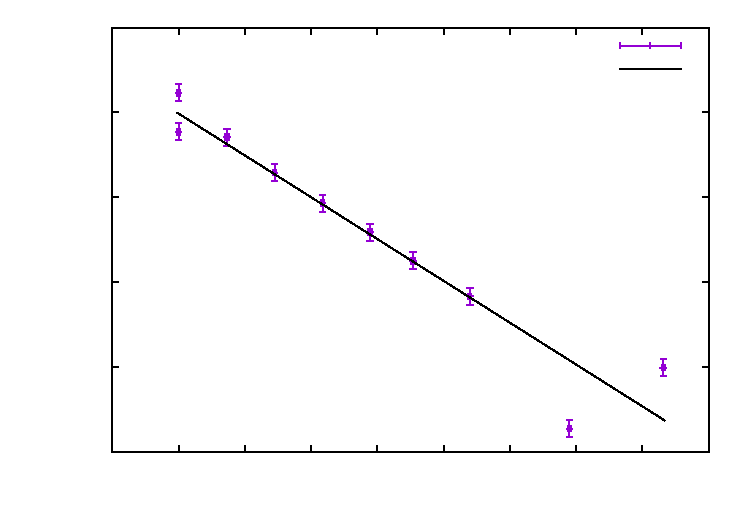
\includegraphics{hoehe}}%
    \gplfronttext
  \end{picture}%
\endgroup
}
		\caption{Höhenabhängigkeit des Drucks: Messwerte und lineare Approximation}
		\label{fig:druckHoehe}
	\end{minipage}
\end{figure}

\section{Tornadoexperiment}
Ein Tornado ist ein Luftwirbel mit fast senkrechter Drehachse, der durch Scherwinde entsteht.
Dies wird in diesem Experiment nachgestellt, indem aus zwei diagonal angeordneten Düsen Luft in entgegengesetzte Richtung ausströmt.

Es gibt verschiedene Modelle, die die Windgeschwindigkeit in Abhängigkeit vom Abstand zur Drehachse beschreiben.
Die hier vorgestellten vernachlässigen die Geschwindigkeit parallel zur Drehachse, befassen sich also nur mit der Tangentialgeschwindigkeit.
Das einfachste Modell ist der \textbf{Rankine-Wirbel}.
Man geht davon aus, dass in der Mitte ein fester Kern mit Radius $R$ ist, der sich mit konstanter Winkelgeschwindigkeit $\omega$ dreht.
Für größere Abstände kann man den Wirbel als Potenzialwirbel beschreiben, die Windgeschwindigkeit fällt mit $r^{-1}$ ab:
\begin{align}
	v(r) = 
	\begin{cases}
		\omega r & \text{falls } r \leq R\\
		\omega \frac{R^2}{r} & \text{falls } r > R\,.\\
	\end{cases}
\end{align}
Diese Funktion ist zwar stetig, aber bei $r=R$ nicht differenzierbar, da dies die Grenze zwischen den beiden Wirbelarten ist.
Physikalisch ist dies nicht so sinnvoll, da es sich in beiden Fällen um das gleiche Fluid handelt und es somit keinen Grund für eine exakte Grenze gibt. 
Das \textbf{Burgers-Rott-Modell}
\begin{align}
	v(r) = \frac{\omega R^2}{r}\left[1-\exp\left(- \frac{r^2}{R^2}\right)\right]
\end{align}
sorgt hingegen für einen sanften Übergang vom Festkörperwirbel zum Potenzialwirbel.
Außerdem erhält man für die Grenzfälle $r \ll R$ sowie $r \gg R$ das Verhalten des Rankine-Wirbels.

Im Experiment wird nun eine Sonde in verschiedenen Höhen und Abständen von der Drehachse in den Tornado gehalten, mit der die Windgeschwindigkeit gemessen wird.
Das Messgerät verfügt über eine zeitliche Mittlung, die benutzt werden sollte.
Um die Messdaten mit den Modellen zu vergleichen, wird die Sonde so herein gehalten, dass man nur die Tangentialgeschwindigkeit misst.
Man erwartet, dass das Geschwindigkeitsprofil höhenunabhängig ist.
In Abbildung \ref{fig:tornado} sind die Messwerte sowie die Modelle mit angepassten Parametern eingezeichnet.
Es wird ein Fehler in der Messung der Windgeschwindigkeit von $\sigma_v = 0.1\,$m/s angenommen.
Beim Fit lässt man jedoch noch einen Parameter $\Delta$ in $r$-Richtung zu, da in der Mitte nie Windstille gemessen wurde -- wie es die Modelle jedoch vorhersagen.
So ist $r_\Delta:=r-\Delta$.
Diese Verschiebung kann zum einen daran liegen, dass die Sonde nicht exakt in der Mitte war.
Zum anderen kann es jedoch sein, dass der Modelltornado leicht schwankt, die Drehachse also nicht ortsfest ist und so über die Mittlung auch darüber gemittelt wird.
Außerdem darf man die Vertikalgeschwindigkeit nicht vernachlässigen, da in diesem Aufbau von unten ständig Luft zugeführt wird.
Wie groß diese Geschwindigkeit ist, wurde allerdings nicht gemessen.
 \begin{figure}[!htb]
	\begin{minipage}{0.5\textwidth}	
		\resizebox{\textwidth}{!}{   		
   		% GNUPLOT: LaTeX picture with Postscript
\begingroup
  \makeatletter
  \providecommand\color[2][]{%
    \GenericError{(gnuplot) \space\space\space\@spaces}{%
      Package color not loaded in conjunction with
      terminal option `colourtext'%
    }{See the gnuplot documentation for explanation.%
    }{Either use 'blacktext' in gnuplot or load the package
      color.sty in LaTeX.}%
    \renewcommand\color[2][]{}%
  }%
  \providecommand\includegraphics[2][]{%
    \GenericError{(gnuplot) \space\space\space\@spaces}{%
      Package graphicx or graphics not loaded%
    }{See the gnuplot documentation for explanation.%
    }{The gnuplot epslatex terminal needs graphicx.sty or graphics.sty.}%
    \renewcommand\includegraphics[2][]{}%
  }%
  \providecommand\rotatebox[2]{#2}%
  \@ifundefined{ifGPcolor}{%
    \newif\ifGPcolor
    \GPcolortrue
  }{}%
  \@ifundefined{ifGPblacktext}{%
    \newif\ifGPblacktext
    \GPblacktexttrue
  }{}%
  % define a \g@addto@macro without @ in the name:
  \let\gplgaddtomacro\g@addto@macro
  % define empty templates for all commands taking text:
  \gdef\gplbacktext{}%
  \gdef\gplfronttext{}%
  \makeatother
  \ifGPblacktext
    % no textcolor at all
    \def\colorrgb#1{}%
    \def\colorgray#1{}%
  \else
    % gray or color?
    \ifGPcolor
      \def\colorrgb#1{\color[rgb]{#1}}%
      \def\colorgray#1{\color[gray]{#1}}%
      \expandafter\def\csname LTw\endcsname{\color{white}}%
      \expandafter\def\csname LTb\endcsname{\color{black}}%
      \expandafter\def\csname LTa\endcsname{\color{black}}%
      \expandafter\def\csname LT0\endcsname{\color[rgb]{1,0,0}}%
      \expandafter\def\csname LT1\endcsname{\color[rgb]{0,1,0}}%
      \expandafter\def\csname LT2\endcsname{\color[rgb]{0,0,1}}%
      \expandafter\def\csname LT3\endcsname{\color[rgb]{1,0,1}}%
      \expandafter\def\csname LT4\endcsname{\color[rgb]{0,1,1}}%
      \expandafter\def\csname LT5\endcsname{\color[rgb]{1,1,0}}%
      \expandafter\def\csname LT6\endcsname{\color[rgb]{0,0,0}}%
      \expandafter\def\csname LT7\endcsname{\color[rgb]{1,0.3,0}}%
      \expandafter\def\csname LT8\endcsname{\color[rgb]{0.5,0.5,0.5}}%
    \else
      % gray
      \def\colorrgb#1{\color{black}}%
      \def\colorgray#1{\color[gray]{#1}}%
      \expandafter\def\csname LTw\endcsname{\color{white}}%
      \expandafter\def\csname LTb\endcsname{\color{black}}%
      \expandafter\def\csname LTa\endcsname{\color{black}}%
      \expandafter\def\csname LT0\endcsname{\color{black}}%
      \expandafter\def\csname LT1\endcsname{\color{black}}%
      \expandafter\def\csname LT2\endcsname{\color{black}}%
      \expandafter\def\csname LT3\endcsname{\color{black}}%
      \expandafter\def\csname LT4\endcsname{\color{black}}%
      \expandafter\def\csname LT5\endcsname{\color{black}}%
      \expandafter\def\csname LT6\endcsname{\color{black}}%
      \expandafter\def\csname LT7\endcsname{\color{black}}%
      \expandafter\def\csname LT8\endcsname{\color{black}}%
    \fi
  \fi
    \setlength{\unitlength}{0.0500bp}%
    \ifx\gptboxheight\undefined%
      \newlength{\gptboxheight}%
      \newlength{\gptboxwidth}%
      \newsavebox{\gptboxtext}%
    \fi%
    \setlength{\fboxrule}{0.5pt}%
    \setlength{\fboxsep}{1pt}%
\begin{picture}(7200.00,5040.00)%
    \gplgaddtomacro\gplbacktext{%
      \csname LTb\endcsname%
      \put(682,704){\makebox(0,0)[r]{\strut{}$2$}}%
      \put(682,1213){\makebox(0,0)[r]{\strut{}$3$}}%
      \put(682,1722){\makebox(0,0)[r]{\strut{}$4$}}%
      \put(682,2231){\makebox(0,0)[r]{\strut{}$5$}}%
      \put(682,2740){\makebox(0,0)[r]{\strut{}$6$}}%
      \put(682,3248){\makebox(0,0)[r]{\strut{}$7$}}%
      \put(682,3757){\makebox(0,0)[r]{\strut{}$8$}}%
      \put(682,4266){\makebox(0,0)[r]{\strut{}$9$}}%
      \put(682,4775){\makebox(0,0)[r]{\strut{}$10$}}%
      \put(814,484){\makebox(0,0){\strut{}$0$}}%
      \put(1479,484){\makebox(0,0){\strut{}$2$}}%
      \put(2145,484){\makebox(0,0){\strut{}$4$}}%
      \put(2810,484){\makebox(0,0){\strut{}$6$}}%
      \put(3476,484){\makebox(0,0){\strut{}$8$}}%
      \put(4141,484){\makebox(0,0){\strut{}$10$}}%
      \put(4807,484){\makebox(0,0){\strut{}$12$}}%
      \put(5472,484){\makebox(0,0){\strut{}$14$}}%
      \put(6138,484){\makebox(0,0){\strut{}$16$}}%
      \put(6803,484){\makebox(0,0){\strut{}$18$}}%
    }%
    \gplgaddtomacro\gplfronttext{%
      \csname LTb\endcsname%
      \put(176,2739){\rotatebox{-270}{\makebox(0,0){\strut{}$v$ [$\frac{\text{m}}{\text{s}}$]}}}%
      \put(3808,154){\makebox(0,0){\strut{}$r$ [cm]}}%
      \csname LTb\endcsname%
      \put(5816,4602){\makebox(0,0)[r]{\strut{}Messwerte}}%
      \csname LTb\endcsname%
      \put(5816,4382){\makebox(0,0)[r]{\strut{}Rankine-Modell}}%
      \csname LTb\endcsname%
      \put(5816,4162){\makebox(0,0)[r]{\strut{}Burgers-Rott-Modell}}%
    }%
    \gplbacktext
    \put(0,0){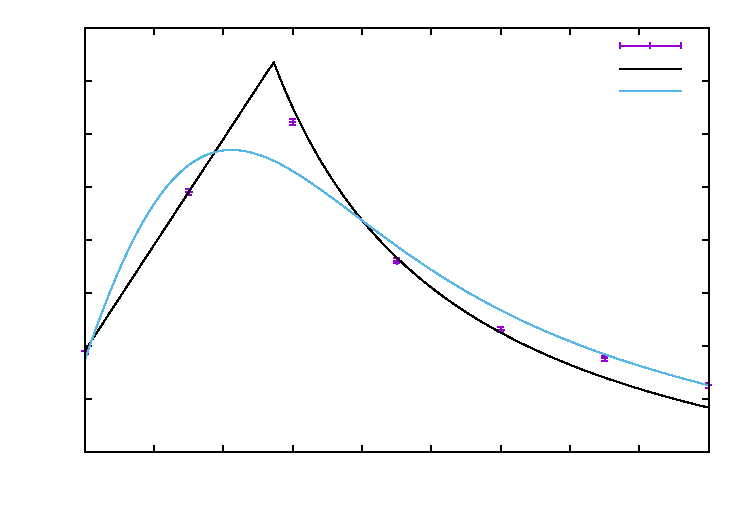
\includegraphics{tornado1}}%
    \gplfronttext
  \end{picture}%
\endgroup
}
   		\caption*{\footnotesize{$h=20\,$cm}}
   \end{minipage}   
   \begin{minipage}{0.5\textwidth}   		
		\resizebox{\textwidth}{!}{   		
   		% GNUPLOT: LaTeX picture with Postscript
\begingroup
  \makeatletter
  \providecommand\color[2][]{%
    \GenericError{(gnuplot) \space\space\space\@spaces}{%
      Package color not loaded in conjunction with
      terminal option `colourtext'%
    }{See the gnuplot documentation for explanation.%
    }{Either use 'blacktext' in gnuplot or load the package
      color.sty in LaTeX.}%
    \renewcommand\color[2][]{}%
  }%
  \providecommand\includegraphics[2][]{%
    \GenericError{(gnuplot) \space\space\space\@spaces}{%
      Package graphicx or graphics not loaded%
    }{See the gnuplot documentation for explanation.%
    }{The gnuplot epslatex terminal needs graphicx.sty or graphics.sty.}%
    \renewcommand\includegraphics[2][]{}%
  }%
  \providecommand\rotatebox[2]{#2}%
  \@ifundefined{ifGPcolor}{%
    \newif\ifGPcolor
    \GPcolortrue
  }{}%
  \@ifundefined{ifGPblacktext}{%
    \newif\ifGPblacktext
    \GPblacktexttrue
  }{}%
  % define a \g@addto@macro without @ in the name:
  \let\gplgaddtomacro\g@addto@macro
  % define empty templates for all commands taking text:
  \gdef\gplbacktext{}%
  \gdef\gplfronttext{}%
  \makeatother
  \ifGPblacktext
    % no textcolor at all
    \def\colorrgb#1{}%
    \def\colorgray#1{}%
  \else
    % gray or color?
    \ifGPcolor
      \def\colorrgb#1{\color[rgb]{#1}}%
      \def\colorgray#1{\color[gray]{#1}}%
      \expandafter\def\csname LTw\endcsname{\color{white}}%
      \expandafter\def\csname LTb\endcsname{\color{black}}%
      \expandafter\def\csname LTa\endcsname{\color{black}}%
      \expandafter\def\csname LT0\endcsname{\color[rgb]{1,0,0}}%
      \expandafter\def\csname LT1\endcsname{\color[rgb]{0,1,0}}%
      \expandafter\def\csname LT2\endcsname{\color[rgb]{0,0,1}}%
      \expandafter\def\csname LT3\endcsname{\color[rgb]{1,0,1}}%
      \expandafter\def\csname LT4\endcsname{\color[rgb]{0,1,1}}%
      \expandafter\def\csname LT5\endcsname{\color[rgb]{1,1,0}}%
      \expandafter\def\csname LT6\endcsname{\color[rgb]{0,0,0}}%
      \expandafter\def\csname LT7\endcsname{\color[rgb]{1,0.3,0}}%
      \expandafter\def\csname LT8\endcsname{\color[rgb]{0.5,0.5,0.5}}%
    \else
      % gray
      \def\colorrgb#1{\color{black}}%
      \def\colorgray#1{\color[gray]{#1}}%
      \expandafter\def\csname LTw\endcsname{\color{white}}%
      \expandafter\def\csname LTb\endcsname{\color{black}}%
      \expandafter\def\csname LTa\endcsname{\color{black}}%
      \expandafter\def\csname LT0\endcsname{\color{black}}%
      \expandafter\def\csname LT1\endcsname{\color{black}}%
      \expandafter\def\csname LT2\endcsname{\color{black}}%
      \expandafter\def\csname LT3\endcsname{\color{black}}%
      \expandafter\def\csname LT4\endcsname{\color{black}}%
      \expandafter\def\csname LT5\endcsname{\color{black}}%
      \expandafter\def\csname LT6\endcsname{\color{black}}%
      \expandafter\def\csname LT7\endcsname{\color{black}}%
      \expandafter\def\csname LT8\endcsname{\color{black}}%
    \fi
  \fi
    \setlength{\unitlength}{0.0500bp}%
    \ifx\gptboxheight\undefined%
      \newlength{\gptboxheight}%
      \newlength{\gptboxwidth}%
      \newsavebox{\gptboxtext}%
    \fi%
    \setlength{\fboxrule}{0.5pt}%
    \setlength{\fboxsep}{1pt}%
\begin{picture}(7200.00,5040.00)%
    \gplgaddtomacro\gplbacktext{%
      \csname LTb\endcsname%
      \put(682,704){\makebox(0,0)[r]{\strut{}$-2$}}%
      \put(682,1383){\makebox(0,0)[r]{\strut{}$0$}}%
      \put(682,2061){\makebox(0,0)[r]{\strut{}$2$}}%
      \put(682,2740){\makebox(0,0)[r]{\strut{}$4$}}%
      \put(682,3418){\makebox(0,0)[r]{\strut{}$6$}}%
      \put(682,4097){\makebox(0,0)[r]{\strut{}$8$}}%
      \put(682,4775){\makebox(0,0)[r]{\strut{}$10$}}%
      \put(1358,484){\makebox(0,0){\strut{}$0$}}%
      \put(2720,484){\makebox(0,0){\strut{}$5$}}%
      \put(4081,484){\makebox(0,0){\strut{}$10$}}%
      \put(5442,484){\makebox(0,0){\strut{}$15$}}%
      \put(6803,484){\makebox(0,0){\strut{}$20$}}%
    }%
    \gplgaddtomacro\gplfronttext{%
      \csname LTb\endcsname%
      \put(176,2739){\rotatebox{-270}{\makebox(0,0){\strut{}$v$ [$\frac{\text{m}}{\text{s}}$]}}}%
      \put(3808,154){\makebox(0,0){\strut{}$r_\Delta$ [cm]}}%
      \csname LTb\endcsname%
      \put(5816,4602){\makebox(0,0)[r]{\strut{}Messwerte}}%
      \csname LTb\endcsname%
      \put(5816,4382){\makebox(0,0)[r]{\strut{}Rankine-Modell}}%
      \csname LTb\endcsname%
      \put(5816,4162){\makebox(0,0)[r]{\strut{}Burgers-Rott-Modell}}%
    }%
    \gplbacktext
    \put(0,0){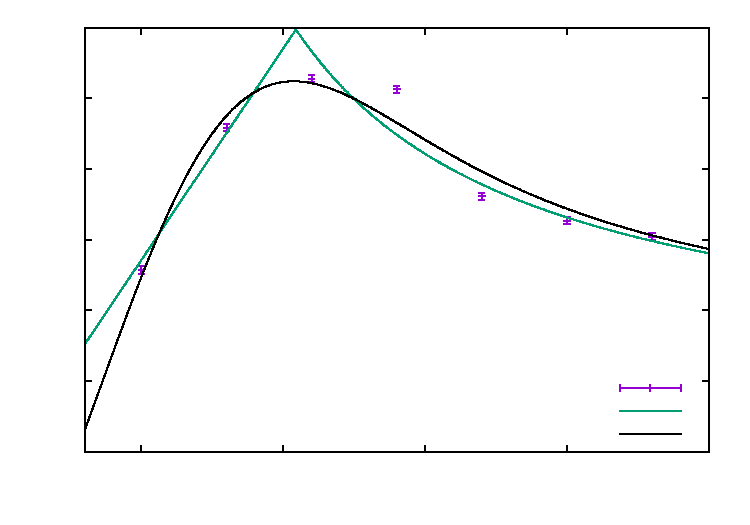
\includegraphics{tornado2}}%
    \gplfronttext
  \end{picture}%
\endgroup
}
   		\caption*{\footnotesize{$h=30\,$cm}}
   \end{minipage}
   \caption{Tornado: Geschwindigkeitsprofil für zwei Höhen $h$}
   \label{fig:tornado}
 \end{figure}
 
\begin{table}[!htb]
 	\centering
 	\begin{tabular}{|c||c|c||c|c|}
 	\hline
 	& \multicolumn{2}{c||}{Rankine} & \multicolumn{2}{c|}{Burgers-Rott}\\
 	& $20\,$cm & $30\,$cm & $20\,$cm & $30\,$cm\\
 	\hline
 	$\omega$ [s$^{-1}$]& $1.15 \pm 0.16$ & $1.2 \pm 0.4$ & $2.3 \pm 0.4$ & $2.2 \pm 0.4$ \\
 	$R$ [cm]               & $7.9 \pm 0.8$ & $8.3 \pm 1.6$ & $5.3 \pm 0.7$ & $6.0 \pm 0.7 $ \\
 	$\Delta$ [cm]         & $3.2 \pm 0.7$ & $2.9 \pm 1.2$ & $1.7  \pm 0.5$ & $ 1.4 \pm 0.5$ \\
 	\hline
 	\end{tabular}
 	\caption{Tornado: gefittete Parameter der beiden Modelle}
 	\label{tab:tornado}
 \end{table} 
 
 In Bezug auf die Höhenunabhängigkeit ist die Geschwindigkeit bei $h=30\,$cm etwas höher.
 Vergleicht man nun aber die Parameter $\omega$, $R$ und $\Delta$ aus dem Fit der Modelle an die Messwerte (Tab. \ref{tab:tornado}), stellt man fest, dass jedes Modell zunächst für die beiden Höhen ähnliche Ergebnisse liefert, jedoch sind Ungenauigkeiten wegen 3 Parametern sehr groß.
Sehr auffällig ist aber, dass die beiden Modelle für die gleichen Messwerte zu sehr unterschiedlichen Parameterwerten gelangen.
So ist $\omega$ bei Burgers-Rott etwa doppelt so groß wie beim Rankine-Wirbel und somit die Verschiebung $\Delta$ und der Kernradius $R$ kleiner.
Dies ist plausibler, da $r_\Delta=0\,$cm nicht so weit von der Mitte weg sein kann.
Zwar passt das Rankine-Modell besser zu den $h=20\,$cm-Werten, das andere Modell kann jedoch beide Messkurven beschreiben -- mit jeweils einem Ausreißer.
 
\end{document}
